\documentclass[11pt,prd,preprint,nofootinbib,amsmath,amssymb]{revtex4-2}

\usepackage[utf8]{inputenc}
\usepackage[T1]{fontenc}
\usepackage{lmodern}
\usepackage{amsmath,amssymb,amsthm,mathtools,bm}
\usepackage{graphicx}
\usepackage{booktabs}
\usepackage{placeins}
\usepackage{xcolor}
\usepackage{siunitx}
\usepackage{hyperref}

\hypersetup{
  colorlinks=true,
  linkcolor=blue,
  citecolor=blue,
  urlcolor=blue
}

\newtheorem{definition}{Definition}
\newtheorem{remark}{Remark}

\newcommand{\Omc}{\Omega_c}
\newcommand{\Omb}{\Omega_b}
\newcommand{\Omm}{\Omega_m}
\newcommand{\Omsel}{\Omega_{\rm sel}}
\newcommand{\Omred}{\Omega_{\rm red}}
\newcommand{\LCDM}{\Lambda{\rm CDM}}
\newcommand{\Mpl}{M_{\rm Pl}}
\newcommand{\dd}{\mathrm d}
\newcommand{\Heff}{H_{\rm eff}}
\newcommand{\Seff}{S_{\rm eff}}
\newcommand{\Geff}{\Gamma_{\rm drain}}

\begin{document}

\title{A CLASS Benchmark for Late-Time Matter-Power Suppression from a Fold-Triggered Dark-Matter Mass Drain}

\author{Liyang Mo}
\affiliation{Independent Researcher}

\date{\today}

\begin{abstract}
We present a CLASS implementation benchmark for a fold-triggered late-time
dark-matter mass-drain mechanism, referred to below as Selection-Fold Dark
Drain. In this mechanism a fold transition in a branch variable $u$ entrains a
scalar $x=\theta/M_{\rm Pl}$ and changes the cold-dark-matter mass as
$m_c(x)=m_{c0}\exp[-\beta_x(x-x_{\rm ini})]$. The resulting late-time matter
drain is tested through a sequence of background, source-level, response-level,
and Newtonian-gauge perturbation checks.

The background bridge reproduces the reconstructed Friedmann branch with
$\max|d\ln H/dN-d\ln E_{\rm Mo}/dN|\simeq7.68\times10^{-10}$. The final
matter-source insertion point is verified by a control test in which a
half-amplitude source shift gives $P_{\mathrm{on}}/P_{\mathrm{off}}=0.25$. In the
fiducial Newtonian-gauge branch we find
$P_{\mathrm{geo}}\simeq0.8971$, $P_{\min}\simeq0.8896$,
$P_{\max}\simeq0.9116$, and a residual shape variation
$\mathrm{tilt}\simeq1.61\%$ over the tested modes.

Interpreted as an amplitude proxy, this corresponds to
$\sqrt{P_{\mathrm{geo}}}\simeq0.947$ and hence to a roughly five-percent
$S_8$-facing suppression. A dense $z=0$ matter-power check gives a
top-hat-windowed amplitude ratio
$\sigma_{8,\rm model}/\sigma_{8,\rm ref}\simeq0.949$, confirming the
geometric proxy at the $2\times10^{-3}$ level. With a Planck 2018 reference amplitude
$S_{8,\mathrm{ref}}=0.831$, the compressed amplitude proxy is
$S_8\simeq0.787$, in the range of published low-redshift weak-lensing
constraints. The calculation is not a gauge-complete Boltzmann closure and
does not constitute a DES/KiDS/HSC/Planck likelihood analysis.
\end{abstract}

\maketitle

\section{Introduction}

Late-time suppression of matter clustering is a recurring target for models
addressing the low-redshift growth amplitude inferred from weak lensing,
galaxy clustering, and redshift-space distortions
\cite{DESY3_3x2pt,DESY3Shear,KiDS1000,HSCY1,HSCY3Shear,eBOSS2020,Heymans2021,Joudaki2020,Alam2017}.
A useful mechanism should satisfy several requirements. It should reduce the
effective matter clustering amplitude at late times, avoid excessive
distortions of the background distance ladder, remain screened or weakly active
at early times, and not introduce uncontrolled scale dependence into the matter
power spectrum.

In this work we study a late-time mechanism that we call the \emph{Selection-Fold Dark Drain}. Its defining chain is
\begin{equation}
\begin{aligned}
U_{\rm sel}(u;\Omega_c)
\;\Longrightarrow\;
u\text{ fold}
\;\Longrightarrow\;
x\text{ entrainment}
\;\Longrightarrow\;
m_c(x)
\\
\;\Longrightarrow\;
\Omega_c\text{ drain}
\;\Longrightarrow\;
P(k),S_8\downarrow .
\end{aligned}
\end{equation}
Here $u(N)$ is a selection-branch coordinate, $x(N)=\theta/M_{\rm Pl}$ is a physical dark scalar, and $N=\ln a$ is the e-fold time.

\begin{figure}[t]
\centering
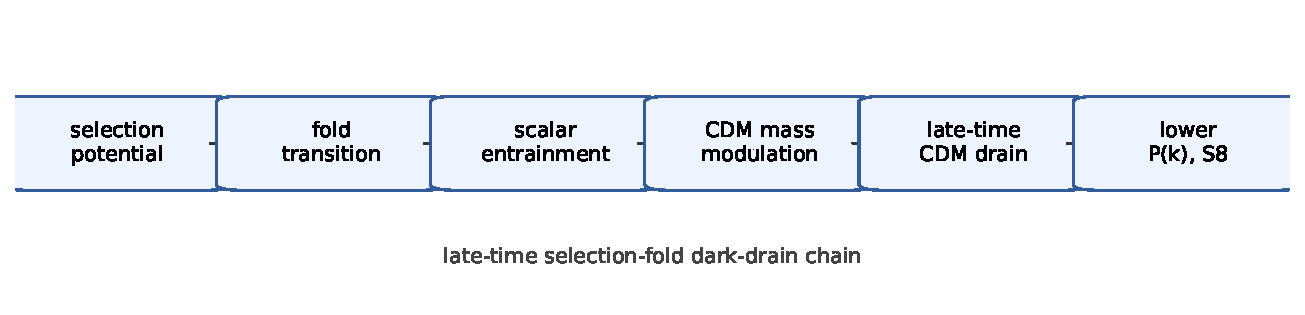
\includegraphics[width=0.95\linewidth]{figures/fig1_mechanism.pdf}
\caption{Selection-fold dark-drain mechanism. A fold transition in the
selection branch coordinate entrains a physical scalar, modulates the
cold-dark-matter mass, drains $\Omega_c$ at late times, and suppresses the
linear matter-power amplitude.}
\label{fig:mechanism}
\end{figure}

This paper focuses on a benchmark implementation rather than a cosmological
data analysis. Its purpose is to establish that the selection-fold mechanism
can be implemented consistently at the background level, that a controlled
effective perturbation bridge can imprint a stable late-time matter-power
suppression into CLASS output without large scale-dependent tilt, and
that a Newtonian-gauge CLASS implementation can register
$(\delta u,\delta x)$, verify the matter-source insertion point, preserve
baseline parity, and admit a bounded final replay while remaining short of
gauge-complete closure.

The presentation follows the calculation. We first define the fold-driven
background model, then construct the CLASS background bridge and the
source-layer matter-power insertion. We next replace the effective source by
quasistatic and dynamic response variants, test the coupled growth response,
and finally evaluate the Newtonian-gauge CLASS branch and its $S_8$-scale
interpretation. Throughout, we distinguish implementation tests from physical
gauge-complete closure and from likelihood-level cosmological inference.

The main results are:
(i) a fold-corrected CLASS background bridge with sub-percent expansion
residuals and a derivative-level consistency check at
$7.68\times10^{-10}$;
(ii) identification and validation of the final CLASS matter-source insertion
chain;
(iii) response-derived and dynamic source replacements with controlled
matter-power tilt;
(iv) a Newtonian-gauge CLASS benchmark reaching
$P_{\mathrm{geo}}\simeq0.8971$ with $\mathrm{tilt}\simeq1.61\%$;
and (v) an $S_8$-facing amplitude proxy of approximately $5.3\%$.

The theoretical role of the selection potential in this work is deliberately
limited. We do not assume a complete microscopic theory of branch selection.
Instead, $U_{\rm sel}$ is used as a local effective potential obtained after
coarse graining over faster boundary, readout, and fluctuation sectors. A
useful operational interpretation is that $U_{\rm sel}$ represents the local
continuum limit of a branch-selection cost that favors dynamically stable,
low-leakage branches with resolvable coarse graining and environmental support.
The cosmological model then
uses the lowest-order fold normal form of this effective potential, with the
CDM abundance acting as the control variable. This places the construction in
the standard logic of effective field theory: the detailed ultraviolet origin
is not fixed, but the allowed low-energy branch dynamics, response scales, and
stability diagnostics are made explicit and tested in CLASS.

\section{Selection-potential motivation}
\label{sec:selection_potential}

We use the selection potential as an effective local free-energy functional
for slow branch variables. Let $X^A(\lambda)$ denote the slow collective
coordinates that remain after coarse graining, and let $b,Y,\zeta$ denote
boundary, readout, and fast fluctuation sectors. Integrating out these sectors
defines an effective action for the slow variables. The term ``selection
potential'' refers only to the local, low-derivative part of this effective
action. This viewpoint is analogous in spirit to the use of coarse-grained
free energies and local effective actions in phase-transition and
effective-field-theory settings
\cite{Wilson1971,WeinbergEFT,LandauLifshitzStat,ArnoldCatastrophe}.
Formally, the path weight is
\begin{equation}
P[X]\propto
\int \mathcal D b\,\mathcal D Y\,\mathcal D\zeta\,
\exp\left[
-\frac{1}{\varepsilon}S_{\rm tot}[X,b,Y,\zeta]
\right],
\end{equation}
and we define
\begin{equation}
\Gamma_{\rm eff}[X]
=
-\varepsilon\log P[X].
\end{equation}
In a low-derivative, local, weak-memory approximation,
\begin{equation}
\Gamma_{\rm eff}[X]
=
\int d\lambda
\left[
\frac12G_{AB}(X)\dot X^A\dot X^B
+
U_{\rm sel}(X)
\right]
+
\Delta\Gamma_{\rm nonlocal}.
\end{equation}

A generic local selection potential may contain terms of the schematic form
\begin{align}
U_{\rm sel}(X)
=&\;
U_0(X)
+\lambda_b\Phi(X)^2
+\lambda_g\left(\mathcal K(X)-\mathcal K_\star\right)^2
\nonumber\\
&+
\frac12\left(O(X)-R\right)^T C^{-1}\left(O(X)-R\right)
-\tau_R\log\det\left(1+\ell^2\mathfrak F(X)\right)
\nonumber\\
&+
\frac{\varepsilon}{2}\log\det{}'\mathcal K_{\rm fluc}(X)
+
\Lambda_{\rm neg}N_-\left(\mathcal K_{\rm fluc}\right)
+\cdots ,
\label{eq:generic_usel}
\end{align}
where $\mathfrak F_{AB}=\partial_AO_i\,C^{-1}_{ij}\,\partial_BO_j$. The terms
in Eq.~\eqref{eq:generic_usel} represent possible local costs and rewards
generated by coarse graining, including boundary anchoring, readout mismatch,
fluctuation stability, and negative-mode penalties.

A complementary operational motivation comes from branch-model selection in
open systems, decoherence theory, Quantum Darwinism, and minimum-description
length model selection
\cite{Zurek2003,Schlosshauer2007,Zurek2009,Rissanen1978,Grunwald2007}.
In such a view, stability, leakage, coarse-graining cost, and environmental
support contribute to an effective branch cost. We use this only to motivate
the signs and roles of local terms in $U_{\rm sel}$, not as an additional
dynamical law.

Equation~\eqref{eq:generic_usel} should be read as a template for the possible
local terms generated by coarse graining, not as a claim that every term is
independently measured in the present cosmological benchmark. The dark-drain
model below uses only the minimal one-dimensional fold sector and its
two-field response completion. The remaining terms provide a bookkeeping
language for stability, readout alignment, fluctuation penalties, and
coarse-graining cost.

A useful bridge to effective field theory is obtained by expanding around a stable selected branch $X_\star$. The Hessian
\begin{equation}
H_{AB}=\nabla_A\nabla_B U_{\rm sel}(X_\star)
\end{equation}
gives the effective mass spectrum through the generalized eigenvalue problem
\begin{equation}
H_{AB}v_n^B=m_n^2G^\star_{AB}v_n^B.
\end{equation}
Thus selected branches are not merely kinematic labels. Their local curvature defines the effective field spectrum.
This is the only aspect of the broader selection picture used later in the
perturbation analysis: the response sector is organized by the curvature and
stability of the selected branch, while the CLASS benchmark tests whether the
resulting effective source can be transmitted to matter power without
large scale dependence.

\section{Two-field selection-fold dark-drain model}
\label{sec:model}

\subsection{Fold potential}

The active selection direction is modeled by the minimal normal form of a
one-dimensional fold transition. Near such a transition, the full
high-dimensional selection landscape is assumed to reduce to one soft branch
coordinate $u$, while the remaining directions are treated as stable or
integrated out. The quartic-minus-quadratic potential below is therefore used
as an effective fold normal form, not as a microscopic ultraviolet potential.

The cosmological mechanism uses a one-dimensional selection branch coordinate $u(N)$ with potential
\begin{equation}
U_{\rm sel}(u;\Omega_c)
=
\frac14u^4-\frac12u^2+J_{\rm eff}(\Omega_c)u.
\label{eq:usel_fold}
\end{equation}
The control variable is
\begin{equation}
J_{\rm eff}(\Omega_c)
=
-J_0\tanh\left[
\frac{1-\Omega_c/\Omega_{\rm tr}}{\sigma_J}
\right].
\label{eq:Jeff}
\end{equation}
The fold critical value of the cubic branch equation is
\begin{equation}
J_{\rm crit}=\frac{2}{3\sqrt3}.
\end{equation}

A key convention identified in the CLASS bridge is that the threshold is not
the naive value $\Omega_{c,\rm ref}a_{\rm tr}^{-3}$, but rather the
fold-corrected value. With the sign convention in Eq.~\eqref{eq:Jeff}, the
benchmark transition is defined by the branch crossing
$J_{\rm eff}=-J_{\rm crit}$ at $a=a_{\rm tr}$. This gives
\begin{equation}
\Omega_{\rm tr}
=
\frac{
\Omega_{c,\rm ref}a_{\rm tr}^{-3}
}{
1-\sigma_J\operatorname{atanh}(J_{\rm crit}/J_0)
}.
\label{eq:fold_corrected_threshold}
\end{equation}
This correction is essential for reproducing the early high-density shoulder of the drain source.

\subsection{Physical scalar and dark-matter drain}

Throughout this subsection, $\Omega_i(N)$ denotes the density component
normalized to the present critical density, not the instantaneous fractional
density divided by $E^2(N)$.

The physical scalar is
\begin{equation}
x(N)=\theta/M_{\rm Pl}.
\end{equation}
It couples to the cold-dark-matter mass through
\begin{equation}
m_c(x)=m_{c0}\exp[-\beta_x(x-x_{\rm ini})].
\label{eq:mass_coupling}
\end{equation}
The cumulative drain is
\begin{equation}
d(N)=\beta_x[x(N)-x_{\rm ini}],
\end{equation}
and the cold-dark-matter density evolves as
\begin{equation}
\Omega_c(N)
=
\Omega_{c,\rm ref}\exp[-3N-d(N)].
\end{equation}
We define the raw drain rate as
\begin{equation}
\Gamma_{\rm raw}=\beta_x x' .
\end{equation}
In the numerical bridge we use the zero-floor transfer prescription
\begin{equation}
\Gamma_{\rm drain}=\max(\Gamma_{\rm raw},0).
\end{equation}
The cold-dark-matter evolution and the transfer equations below use this
$\Gamma_{\rm drain}$:
\begin{equation}
\Omega_c'=-(3+\Gamma_{\rm drain})\Omega_c.
\label{eq:omega_c_drain}
\end{equation}

The drained energy is routed into a selection-like dark component and a fast-redshifting component:
\begin{align}
\Omega_{\rm sel}'
&=
-3(1+w_{\rm sel})\Omega_{\rm sel}
+\epsilon_{\rm DE}\Gamma_{\rm drain}\Omega_c,
\\
\Omega_{\rm red}'
&=
-3(1+w_{\rm red})\Omega_{\rm red}
+
(1-\epsilon_{\rm DE})\Gamma_{\rm drain}\Omega_c,
\end{align}
with
\begin{equation}
w_{\rm sel}=-1,
\qquad
w_{\rm red}=1.
\end{equation}
The drain prescription checks used to define the fiducial transfer rule are
summarized in Table~\ref{tab:drain_prescription_robustness}.

\begin{table*}[t]
\centering
\small
\resizebox{\textwidth}{!}{%
\begin{tabular}{llll}
\toprule
Prescription & Drain behavior & Suppression response & Interpretation \\
\midrule
Zero floor $\max(\Gamma_{\rm raw},0)$ & fiducial late-time drain & fiducial output & used in main runs \\
Signed $\Gamma_{\rm raw}$ & bounded; no runaway reversal & consistent qualitative behavior & not a hard-floor artifact \\
Smooth zero floor & stable late-time drain & consistent qualitative behavior & smooth replacement check \\
Naive softplus & high-$z$ leakage & rejected & not used in benchmark \\
\bottomrule
\end{tabular}
}
\caption{Drain-prescription robustness summary. The comparison records which
transfer prescriptions were retained or rejected in the benchmark construction.
The zero-floor prescription is used in the main runs; the signed and smooth
zero-floor variants provide prescription-level sanity checks, while the naive
softplus variant is excluded because it introduces unwanted high-redshift
leakage.}
\label{tab:drain_prescription_robustness}
\end{table*}

\subsection{Two-field dynamics}

The full two-field potential is
\begin{equation}
U_{\rm total}(u,x;\Omega_c)
=
U_{\rm sel}(u;\Omega_c)
+
\frac12m_L^2(x-u)^2
+
\frac12m_x^2(x-x_{\rm ini})^2.
\end{equation}
The first-order relaxation dynamics used in the benchmark are
\begin{align}
u'
&=
-\Gamma_u
\left[
u^3-u+J_{\rm eff}
-
m_L^2(x-u)
\right],
\label{eq:u_rhs}
\\
x'
&=
-\Gamma_x
\left[
m_L^2(x-u)+m_x^2(x-x_{\rm ini})
\right].
\label{eq:x_rhs}
\end{align}
A direct fit to the standalone background table confirms the benchmark values
\begin{equation}
\Gamma_u\simeq12,
\qquad
\Gamma_x\simeq200,
\qquad
m_L^2\simeq2,
\qquad
m_x^2\simeq0.
\end{equation}

\subsection{Relation to interacting dark-sector benchmarks}

The present construction is related to interacting dark-energy and
coupled-dark-matter scenarios, in which energy exchange or scalar-mediated
forces modify the late-time growth history
\cite{Amendola2000,Wetterich1995,Koivisto2005,Valiviita2008,Gavela2009,Bean2008}.
The distinguishing feature here is that the interaction is not introduced as a
constant coupling or as a prescribed phenomenological transfer function. It is
triggered by a fold-like branch transition controlled by the CDM abundance,
which then entrains the scalar controlling the dark-matter mass. In this sense
the model is best viewed as a CLASS benchmark for a transition-triggered
dark-sector drain, rather than as a completed likelihood-level interacting
dark-energy model.
Table~\ref{tab:parameter_roles} summarizes which quantities are physical
dark-sector inputs, effective bridge parameters, numerical normalizations, or
diagnostic-only coordinates.

\begin{table*}[t]
\centering
\small
\resizebox{\textwidth}{!}{%
\begin{tabular}{llll}
\toprule
Parameter & Role & Fixed by & Status \\
\midrule
$J_0$ & fold amplitude & benchmark choice & dark-sector benchmark input \\
$a_{\rm tr}$ & activation epoch & background source alignment & dark-sector benchmark input \\
$\sigma_J$ & transition width & background source alignment & dark-sector benchmark input \\
$\beta_x$ & CDM mass-drain strength & background drain normalization & dark-sector benchmark input \\
$\epsilon_{\rm DE}$ & drain routing fraction & standalone benchmark & phenomenological input \\
$m_L^2,m_x^2$ & two-field locking and scalar stiffness & background replay & model input \\
$\Gamma_u,\Gamma_x$ & relaxation rates & background replay & effective dynamics \\
$C_{\rm drain}$ & effective source amplitude & source bridge scan & bridge parameter \\
$C_x$ & response-source amplitude & response bridge scan & bridge parameter \\
$p$ & response gate power & response bridge scan & phenomenological gate \\
$g_{\rm grow}$ & source-to-growth projection gain & coupled replay calibration & bridge calibration \\
$\Gamma_{\rm mult}$ & response relaxation normalization & local envelope scan & numerical normalization \\
$X_{\rm norm}$ & online response normalization & bounded CLASS replay & numerical normalization \\
$\Lambda_{\rm met}$ & metric-source diagnostic coordinate & finite metric audit & diagnostic only \\
\bottomrule
\end{tabular}
}
\caption{Parameter roles in the benchmark. The table separates physical
dark-sector inputs from effective bridge parameters, numerical normalization
choices, and diagnostic-only quantities.}
\label{tab:parameter_roles}
\end{table*}

\section{Standalone benchmark}
\label{sec:standalone}

The main standalone benchmark uses
\begin{align}
J_0&=0.8,
&
\epsilon_{\rm DE}&=0.16,
&
\Gamma_u&=12,
\nonumber\\
\Gamma_x&=200,
&
m_L^2&=2.0,
&
m_x^2&=0.
\end{align}
The original standalone bridge gives
\begin{align}
d_{\rm transfer,final}&\simeq0.069052,
&
d_{\rm field,final}&\simeq0.069059,
\\
\Omega_{c0}^{\rm eff}&\simeq0.242652,
&
\Omega_{m0}^{\rm eff}&\simeq0.292652,
\\
\Omega_{\rm sel,0}&\simeq0.043877,
&
\Omega_{\rm red,0}&\simeq1.536\times10^{-3},
\\
\Omega_{\Lambda,{\rm model}}&\simeq0.661845,
&
\max|x-u|&\simeq0.02849.
\end{align}
The effective growth replay gives
\begin{equation}
S_8^{\rm proxy}
\simeq
0.94710,\ 0.94797,\ 0.95056,\ 0.95489,\ 0.96097
\end{equation}
for
\begin{equation}
\beta_{\rm eff}=0,\ 0.05,\ 0.10,\ 0.15,\ 0.20.
\end{equation}
This demonstrates that the benchmark remains in a few-percent suppression regime under activated fifth-force-like corrections.

\section{CLASS background bridge}
\label{sec:class_background}

\subsection{Bridge implementation}

We implemented a background-only bridge in CLASS \cite{CLASS}, in the same
Boltzmann-solver ecosystem as CAMB and its modified-gravity extensions
\cite{CAMB,EFTCAMB,hiCLASS}. The bridge evolves $u$, $x$, $\Omega_c$,
$\Omega_{\rm sel}$, $\Omega_{\rm red}$, and $d_{\rm transfer}$, and outputs
diagnostic columns including
\begin{equation}
u,\ x,\ \Gamma_{\rm drain},\ \Omega_c,\ \Omega_{\rm sel},\ \Omega_{\rm red},\ d_{\rm transfer},
\end{equation}
as well as the reconstructed Friedmann branch
\begin{equation}
E_{\rm Mo}^2(N)
=
\Omega_b(N)+\Omega_r(N)+\Omega_c(N)+\Omega_{\rm sel}(N)+\Omega_{\rm red}(N)+\Omega_\Lambda^{\rm Mo}.
\end{equation}
Here the subscript ``Mo'' labels the reconstructed model branch used as the
background handoff target.
In the latest audit branch we further exposed internal RHS diagnostics
\begin{equation}
J_{\rm eff},\ dU_du,\ dU_dx,\ u'_{\rm rhs},\ x'_{\rm rhs},
\end{equation}
and echo columns for
\begin{equation}
\Omega_c',\ \Omega_{\rm sel}',\ \Omega_{\rm red}',\ d_{\rm transfer}',
\end{equation}
to verify that integrated derivatives and printed diagnostics are generated from the same code path.

A gated handoff was introduced:
\begin{equation}
H_{\rm CLASS}\leftarrow H_{\rm Mo}
\end{equation}
when the Mo bridge is active. This lowers the main $H(z)$ mismatch relative to the standalone target.

\subsection{Source-shape alignment}

Before implementing the fold-corrected threshold, the CLASS bridge missed the early high-density shoulder of the drain source. The key diagnostic was the source budget
\begin{equation}
I_{\rm source}
=
\int \Gamma_{\rm drain}(N)\Omega_c(N)\,dN.
\end{equation}
The standalone bridge has
\begin{equation}
I_{\rm source}^{\rm target}\simeq0.274232,
\qquad
\langle\Omega_c\rangle_\Gamma\simeq3.971.
\end{equation}
After implementing Eq.~\eqref{eq:fold_corrected_threshold} and locally refining $(a_{\rm tr},\sigma_J,\beta_x)$, we find a source-shape bridge point
\begin{equation}
a_{\rm tr}=0.335,
\qquad
\sigma_J=0.78,
\qquad
\beta_x=0.0274125,
\end{equation}
with
\begin{equation}
I_{\rm source}\simeq0.2680,
\qquad
z_{\rm peak}\simeq0.9024,
\qquad
{\rm area}(N<-1.2)\simeq0.0958.
\end{equation}
This is close to the standalone target
\begin{equation}
I_{\rm source}^{\rm target}\simeq0.2742,
\qquad
z_{\rm peak}^{\rm target}\simeq0.909,
\qquad
{\rm area}_{N<-1.2}^{\rm target}\simeq0.104.
\end{equation}

\subsection{Development audits and threshold convention}

Several implementation audits were used to isolate the source of the early
background mismatch. Start-time tests and derivative-variable checks ruled out
initialization and $d/d\ln a$ convention errors. A single-source RHS helper was
then introduced so that the background integrator and diagnostic output shared
the same Mo-sector derivative path, reducing RHS parity residuals to the
$10^{-5}$--$10^{-4}$ level.

The remaining source-budget discrepancy was traced to the control mapping in
$J_{\rm eff}(\Omega_c)$. Direct inversion of the benchmark control trajectory
showed that the transition threshold must use the fold-corrected convention in
Eq.~\eqref{eq:fold_corrected_threshold}, rather than the naive
$\Omega_{c,\rm ref}a_{\rm tr}^{-3}$ value. After this correction, the CLASS
bridge recovers the early source shoulder and provides the benchmark
background used in the later perturbation and response stages. The detailed
audit trail is retained in the reproducibility manifest rather than repeated
in the main text.

\subsection{Background closure}

The main consistency checks for the benchmark background are summarized in
Table~\ref{tab:background_consistency}.

\begin{table*}[t]
\centering
\small
\begin{tabular}{p{0.16\textwidth}p{0.42\textwidth}p{0.18\textwidth}p{0.18\textwidth}}
\toprule
Object & Test & Result & Interpretation \\
\midrule
$H(z)$ & relative residual vs reconstructed branch & $5.56\times10^{-4}$ & below $10^{-3}$ \\
$I(z)$ & line-of-sight integral residual, $z>0$ & $4.02\times10^{-4}$ & below $10^{-3}$ \\
$d\ln H/dN$ & derivative residual vs reconstructed branch & $7.68\times10^{-10}$ & derivative-level agreement \\
Geometry columns & optional CLASS synchronization columns & $3\times10^{-3}$ level & secondary check \\
\bottomrule
\end{tabular}
\caption{Summary of the CLASS background bridge consistency checks. The main
expansion and line-of-sight integral are below the $10^{-3}$ level, while
optional geometry and time columns provide a secondary synchronization check.}
\label{tab:background_consistency}
\end{table*}

The benchmark candidate is evaluated with the reconstructed-Friedmann handoff enabled and
with bridge parameters
\begin{equation}
a_{\rm tr}=0.335,\quad \sigma_J=0.78,\quad \beta_x=0.0274125.
\end{equation}
In addition, a derivative self-consistency audit gives
\begin{equation}
\max\left|\,\frac{d\ln H}{dN}-\frac{d\ln E_{\rm Mo}}{dN}\right|
\simeq 7.68\times10^{-10},
\end{equation}
showing that the handed-off $H$ column and the reconstructed Friedmann branch are numerically indistinguishable at the derivative level.

For optional geometry/time columns, we use corrected geometric relations
$D_C\propto I$, $D_A\propto I/(1+z)$, $D_L\propto (1+z)I$, and an affine fit
$\eta\simeq A+B\,I$, with low-$z$ and ultra-high-$z$ tails treated separately in diagnostics.
This confirms that the central bridge requirement is the $(H,I)$ pair, while built-in
geometry/time columns are a secondary synchronization layer.

\begin{figure}[t]
\centering
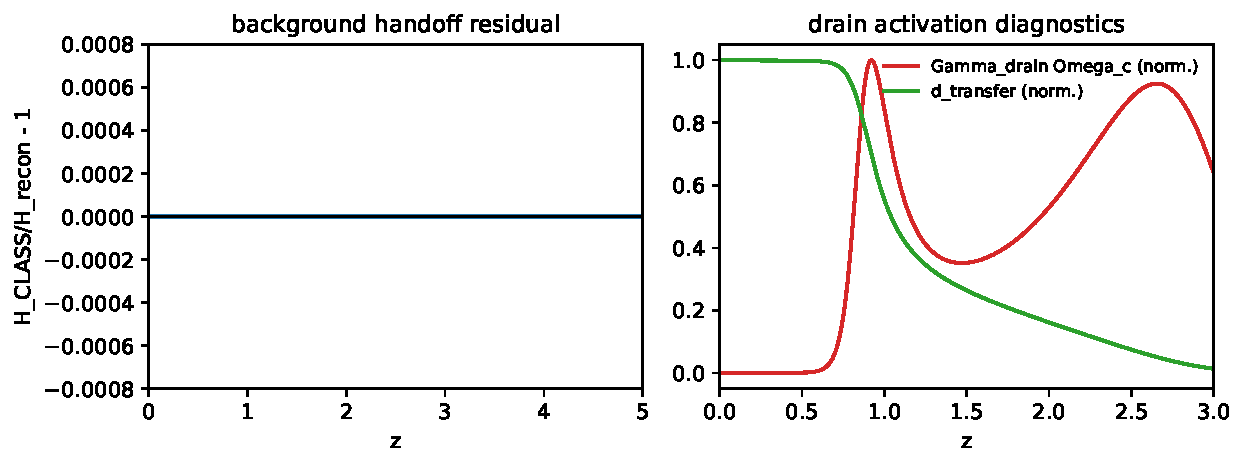
\includegraphics[width=0.95\linewidth]{figures/fig2_background_bridge.pdf}
\caption{Background bridge diagnostics. The left panel shows the relative
handoff residual between the CLASS background and the reconstructed
Friedmann branch. The right panel shows normalized drain-source and
cumulative-transfer diagnostics, illustrating the late-time activation window
used by the perturbation benchmarks.}
\label{fig:background_bridge}
\end{figure}

\section{Effective perturbation bridge}
\label{sec:effective_perturbation}

\subsection{Standalone effective replay}

Before modifying the CLASS perturbation output, we replayed the effective subhorizon growth equations using the benchmark CLASS background. The two-fluid replay evolves CDM and baryon growth variables with an activated fifth-force-like correction
\begin{equation}
\mu_x(k,N)
=
1+
2\beta_{\rm eff}^2A_x(N)
\frac{k^2}{k^2+a^2m_{\rm eff}^2(N)},
\end{equation}
where
\begin{equation}
m_{\rm eff}^2/H_0^2=M_0^2+M_1^2A_x(N).
\end{equation}
Under the internal convention $\Omega_{m0}^{\Lambda{\rm CDM}}=0.31$, all
32 mixed and CDM-only replay branches satisfy the stated stability criteria,
with
\begin{equation}
S_8^{\rm proxy}\simeq0.95064\text{--}0.95709,
\qquad
|\text{tilt}|\sim0.002\%.
\end{equation}
A stress convention $\Omega_{m0}^{\Lambda{\rm CDM}}=0.315$ initially fails the hard $S_8\ge0.94$ lower cut in some branches, but passes under $S_8\ge0.935$. This identifies the effect as a normalization stress sensitivity, not a scale-dependent instability.
For completeness, we performed an explicit convention calibration replay. The
official branch with $\Omega_{m0}^{\Lambda{\rm CDM}}=0.31$ satisfies the
criteria across all 32 tested branches. A stress branch including
$\Omega_{m0}^{\Lambda{\rm CDM}}=0.315$ also satisfies the relaxed criterion
$S_8\ge0.935$ across all 64 tested branches. Therefore the previous
partial-fail pattern at fixed $S_8\ge0.94$ is a convention-threshold effect,
not a dynamical instability.

\subsection{CLASS source-chain tracing}

A direct Newtonian-gauge Euler hook was first tested:
\begin{equation}
\dot\theta_c
=
-(1+\Gamma_N)\mathcal H\theta_c
+
\mu_{\rm eff}\,{\rm metric\_euler}.
\end{equation}
Although the hook executed, it did not affect the final $P(k)$ output. We
therefore traced the CLASS matter-power source chain and verified that the
Fourier read-side source array is the final matter-power insertion point. To
exclude stale-output artifacts, we repeatedly regenerated the off/on comparison
products before each test. A read-side source-response control that scaled the
relevant matter source by a factor of $0.5$ produced the expected
\begin{equation}
P_{\mathrm{on}}(k)/P_{\mathrm{off}}(k)=0.25
\end{equation}
across the sampled $k$ values. This identifies the Fourier read-side chain as
the final $mPk$ insertion point.

We then performed write/read memory-instance tracing at matched grid points.
For matched time and wavenumber samples, the stored perturbation-source value
and the Fourier-read value agree pointwise. Hence the effective chain from the
perturbation source array to final $mPk$ is directly verified.

Finally, a pointwise source-bias sanity test applied only on a restricted
low-$k$ grid subset gives
\begin{equation}
P_{\mathrm{on}}/P_{\mathrm{off}}=0.25
\end{equation}
for low-$k$ sampled points while higher-$k$ sampled points remain unchanged.
This resolves the earlier apparent contradiction from broad but non-pointwise
diagnostics and confirms that source-layer perturbation insertions are
operational.

Pointwise source-bias tests confirmed that modifying the matter perturbation
source propagates exactly into the final $mPk$ output. This motivated an
intermediate effective source-layer bridge.

\subsection{Gauge-split perturbation access}

Before any physical perturbation insertion, we performed a hook-only
reconnaissance of the perturbation equations. The audit confirms that the CDM
perturbation equations are gauge-split in the standard CLASS form:
\begin{align}
\delta_c'&=-(\theta_c+\text{metric\_continuity}),\qquad
\theta_c'=-\mathcal H\theta_c+\text{metric\_euler}
\quad (\text{newtonian}),\\
\delta_c'&=-\text{metric\_continuity},\qquad \theta_c\equiv0
\quad (\text{synchronous}).
\end{align}
The velocity index for CDM is defined only in Newtonian gauge, while synchronous
gauge uses the gauge condition $\theta_c=0$. This reconnaissance fixes the
gauge scope of the effective bridge: the present implementation is
Newtonian-first, while a synchronous-consistent closure is left for future work.

\subsection{Effective source-layer bridge}

We define an effective source multiplier
\begin{equation}
\delta_m^{\rm source}
\rightarrow
\Seff(N,k)\,\delta_m^{\rm source}.
\end{equation}
The minimal form used in this work is
\begin{equation}
\Seff(N,k)
=
1
-
A_{\rm drain}A_x(N)
+
A_\mu A_x(N)
\frac{k^2}{k^2+a^2H_0^2M_0^2}.
\label{eq:seff}
\end{equation}
Here
\begin{equation}
A_x(N)=\frac{d_{\rm transfer}(N)}{d_{\rm transfer}(0)}.
\end{equation}
The implementation also preserves a constant-source fallback.

A diagnostic constant multiplier $\Seff=0.98$ gives
\begin{equation}
P(k)_{\rm on}/P(k)_{\rm off}=(0.98)^2=0.9604
\end{equation}
at all tested $k$, confirming that the source-layer insertion is stable.

\section{Matter-power results}
\label{sec:results}

For a set of sampled wavenumbers $k_j$, we summarize the matter-power ratio by
\begin{equation}
P_{\mathrm{geo}}
=
\exp\left[
\frac{1}{N_k}
\sum_{j=1}^{N_k}
\ln\left(\frac{P_{\mathrm{on}}(k_j)}{P_{\mathrm{ref}}(k_j)}\right)
\right].
\end{equation}
We denote by $P_{\min}$ and $P_{\max}$ the minimum and maximum of the same
ratio over the sampled $k$ range. The quoted residual scale dependence is
\begin{equation}
\mathrm{tilt}
=
100
\max_j
\left|
\frac{P_{\mathrm{on}}(k_j)/P_{\mathrm{ref}}(k_j)}
{P_{\mathrm{geo}}}
-1
\right|\%.
\end{equation}

\subsection{Calibration scan}

We scanned
\begin{align}
A_{\rm drain}&=0.015,\ 0.020,\ 0.025,\ 0.030,
\\
A_\mu&=0,\ 0.003,\ 0.005,\ 0.008,
\\
M_0&=10,\ 30,\ 100,
\end{align}
with $M_1=0$. The scan contains 48 points; 43 satisfy the baseline diagnostic
criteria and 13 also satisfy the stricter ideal-window criteria.
The best conservative points have
\begin{equation}
A_{\rm drain}=0.020,
\qquad
A_\mu=0,
\end{equation}
with
\begin{equation}
P(k)/P_{\mathrm{off}}=0.9604
\end{equation}
uniformly across
\begin{equation}
k=0.01,\ 0.03,\ 0.10,\ 0.30\ h\,{\rm Mpc}^{-1}.
\end{equation}
A representative mild $k$-dependent point is
\begin{equation}
A_{\rm drain}=0.025,
\qquad
A_\mu=0.005,
\qquad
M_0=10,
\end{equation}
which gives
\begin{equation}
P(k)/P_{\mathrm{off}}\simeq0.9594\text{--}0.9604
\end{equation}
and a tilt of only
\begin{equation}
0.0127\%.
\end{equation}

\subsection{Representative points}

We use three representative points, summarized in
Table~\ref{tab:source_layer_representatives}.
\begin{table*}[t]
\centering
\scriptsize
\setlength{\tabcolsep}{2.5pt}
\resizebox{\textwidth}{!}{%
\begin{tabular}{lcccccccccc}
\toprule
case & $A_{\mathrm{drain}}$ & $A_{\mu}$ & $M_0$ &
$P_{0.01}/P_{\mathrm{off}}$ &
$P_{0.03}/P_{\mathrm{off}}$ &
$P_{0.10}/P_{\mathrm{off}}$ &
$P_{0.30}/P_{\mathrm{off}}$ &
$\min_{z=0\sim2}P/P_{\mathrm{off}}$ &
$\max_{z=0\sim2}P/P_{\mathrm{off}}$ &
max $|\mathrm{tilt}|$ (\%) \\
\midrule
conservative & 0.020 & 0.000 & 10 & 0.9604 & 0.9604 & 0.9604 & 0.9604 & 0.9604 & 0.9935 & $\approx0$ \\
mild $k$-dependent & 0.025 & 0.005 & 10 & 0.9594 & 0.9603 & 0.9604 & 0.9604 & 0.9594 & 0.9935 & 0.01 \\
boundary & 0.030 & 0.000 & 10 & 0.9409 & 0.9409 & 0.9409 & 0.9409 & 0.9409 & 0.9903 & $\approx0$ \\
\bottomrule
\end{tabular}
}
\caption{Representative source-layer effective bridge points. The conservative benchmark gives scale-independent suppression at $z=0$, the mild benchmark introduces only tiny $k$-dependence, and the boundary point illustrates low-redshift amplitude over-suppression.}
\label{tab:source_layer_representatives}
\end{table*}


\subsection{Redshift stability}

The representative points were tested at
\begin{equation}
z=0,\ 0.5,\ 1,\ 2.
\end{equation}
The conservative point gives
\begin{align}
P(k)/P_{\mathrm{off}}
&=
0.9604
\quad (z=0),
\\
&\simeq0.9605
\quad (z=0.5),
\\
&\simeq0.9780
\quad (z=1),
\\
&\simeq0.9935
\quad (z=2),
\end{align}
with negligible tilt at all tested redshifts.

The mild $k$-dependent point gives
\begin{equation}
P(k)/P_{\mathrm{off}}\simeq0.9594\text{--}0.9604
\end{equation}
at $z=0$, with maximum tilt
\begin{equation}
0.0127\%.
\end{equation}
The tilt decreases to
\begin{equation}
2.3\times10^{-4}\%
\end{equation}
by $z=2$.

The boundary point gives
\begin{equation}
P(k)/P_{\mathrm{off}}\simeq0.9409
\end{equation}
at $z=0$, rising to
\begin{equation}
0.9903
\end{equation}
by $z=2$. It is therefore a low-redshift amplitude over-suppression boundary, not a large-tilt boundary.

\begin{figure}[t]
\centering
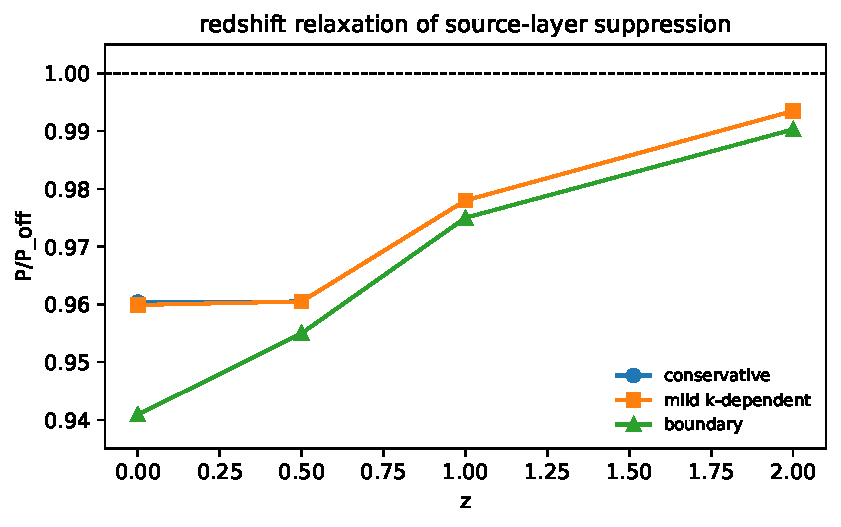
\includegraphics[width=0.72\linewidth]{figures/fig3_pk_redshift.pdf}
\caption{Redshift relaxation of representative source-layer matter-power
suppression. The conservative and mild benchmarks give smooth late-time
suppression and relax toward unity by $z\simeq2$; the boundary point is an
amplitude boundary rather than a scale-tilt pathology.}
\label{fig:pk_redshift}
\end{figure}

\subsection{Quasistatic response-derived source bridge}

To move beyond a purely hand-tuned source multiplier, we constructed a response-background dataset from the benchmark CLASS background output and analyzed a quasi-static two-field response kernel. The background Hessian
\begin{equation}
H=
\begin{pmatrix}
H_{uu} & H_{ux}\\
H_{xu} & H_{xx}
\end{pmatrix}
\end{equation}
shows a short fold-soft interval with negative determinant/eigenvalue support. Quantitatively, the negative-eigenvalue fraction is
\begin{equation}
f_{\lambda_{\min}(H)<0}\simeq 0.0078,
\end{equation}
localized around
\begin{equation}
z\simeq 0.91\text{--}1.46.
\end{equation}
This soft interval is physically expected near a fold transition.

We then considered the finite-$k$ response kernel
\begin{equation}
K=H+Q_k e_xe_x,
\qquad
Q_k\propto \frac{k^2}{a^2H_0^2},
\end{equation}
with regularized/damped variants as controls. Over the tested observational window
\begin{equation}
k=0.01,\ 0.03,\ 0.10,\ 0.30\ h\,{\rm Mpc}^{-1},
\end{equation}
the kernel is lifted to non-negative minimum eigenvalues, i.e. the fold soft mode is stabilized by finite-gradient stiffness. Damping further reduces stiffness modestly but does not change the qualitative conclusion.
In this sense, the data favor a ``soft-but-regularized'' picture: the bare fold sector is locally soft, but the finite-gradient term keeps the tested response kernel invertible over the observational $k$ window. Numerically, the bare Hessian reaches a modest peak condition number $\sim 7.1\times10^3$, while the response kernel is non-negative but extremely stiff (typical condition numbers $\sim10^{30}$--$10^{33}$), motivating normalized-response and clipping safeguards in the prototype scan.

Using the response-derived ansatz
\begin{equation}
S_{\rm phys}(N,k)=1-C_{\rm drain}A_x(N)+C_x\widehat R_x(N,k),
\end{equation}
with normalized response $\widehat R_x$ and clipping safeguards, we ran an 84-point standalone prototype scan:
\begin{equation}
4\ (C_{\rm drain})\times 7\ (C_x)\times 3\ ({\rm kernel})=84.
\end{equation}
The scan finds broad stable regions. For each kernel branch, 25/28 points
satisfy the baseline criteria and 9/28 also satisfy the stricter ideal-window
criteria, with the best point at
\begin{equation}
C_{\rm drain}=0.020,\quad C_x=0,
\end{equation}
recovering
\begin{equation}
P_{\rm ratio}(z=0)\simeq0.9604
\end{equation}
and negligible tilt, with zero clipping in top rows. This supports the interpretation that the effective source-layer bridge can be promoted to a response-derived prototype without introducing large $k$-shape distortions.

\subsection{Source-layer and response-bridge comparison}

To consolidate the development chain, we assembled a direct comparison between
the source-layer bridge and the response-derived bridge, summarized in
Table~\ref{tab:response_bridge_comparison}.
\begin{table*}[t]
\centering
\small
\resizebox{\textwidth}{!}{%
\begin{tabular}{lcccc}
\hline
case & key parameters & $f_{\rm resp}(z=0)$ & $\min_{z,k}P/P_{\rm off}$ & max $|\mathrm{tilt}|$ (\%) \\
\hline
source-layer conservative & $A_{\rm drain}=0.020,\ A_\mu=0$ & 0 & 0.9604 & 0.0000 \\
source-layer mild $k$-dependent & $A_{\rm drain}=0.025,\ A_\mu=0.005,\ M_0=10$ & 0 & 0.9594 & 0.0127 \\
response-derived robust & $p=3.25,\ C_{\rm drain}=0.014,\ C_x=0.015$ & 0.0619 & 0.9451 & 0.3100 \\
response-derived stress & $p=3.25,\ C_{\rm drain}=0.014,\ C_x=0.017$ & 0.0696 & 0.9415 & 0.3514 \\
\hline
\end{tabular}
}
\caption{Source-layer effective bridge versus gated response-derived bridge.}
\label{tab:response_bridge_comparison}
\end{table*}


The source-layer bridge establishes that an effective correction can stably
imprint the target suppression into CLASS matter power without large
scale-dependent tilt. The response-derived bridge then introduces a correction
from the two-field fold kernel with a late-time activation gate. The robust
gated benchmark
\begin{equation}
G_R=A_x^{3.25},\qquad
C_{\rm drain}=0.014,\qquad
C_x=0.015
\end{equation}
gives
\begin{equation}
f_{\rm resp}(z=0)\simeq0.0619,\quad
\min_{z,k}P/P_{\mathrm{off}}\simeq0.9451,\quad
\mathrm{tilt}\simeq0.31\%,
\end{equation}
with zero clipping. A higher-response stress point with $C_x=0.017$ raises $f_{\rm resp}(z=0)$ to $\sim0.0696$ but lowers the all-redshift floor to $\sim0.9415$, indicating the onset of the safe-window boundary.

\subsection{Dynamic-response calibration}

Before modifying CLASS perturbation equations, we tested a standalone first-order dynamic prototype for
\begin{equation}
\eta_u=\frac{\delta u}{\delta_c},
\qquad
\eta_x=\frac{\delta x}{\delta_c},
\end{equation}
with damped response-kernel coefficients matched to the response-derived
benchmark branch. For each sampled mode
\begin{equation}
k=0.01,\ 0.03,\ 0.10,\ 0.30\ h\,{\rm Mpc}^{-1},
\end{equation}
we evolved the dynamic system on $N\in[-8,0]$ and compared $\eta_x(N,k)$ against the quasistatic kernel response $R_x^{\rm QS}(N,k)$.

The prototype is numerically stable for all tested modes and initializations. The dynamic response tracks the quasistatic shape with high correlation,
\begin{equation}
{\rm corr}\!\left(\eta_x,R_x^{\rm QS}\right)\simeq0.993\text{--}0.997,
\end{equation}
and moderate relative error,
\begin{equation}
{\rm rms\_rel}\!\left(\eta_x-R_x^{\rm QS}\right)\simeq0.097\text{--}0.129.
\end{equation}
At late time ($z=0$), the amplitude ratio is close to unity,
\begin{equation}
\eta_x/R_x^{\rm QS}\simeq1.042,
\end{equation}
while by $z=1$ it increases to
\begin{equation}
\eta_x/R_x^{\rm QS}\simeq1.18.
\end{equation}
This behavior supports the dynamic-response benchmark: the dynamic prototype reproduces the quasistatic response pattern with controlled residual bias, but does not yet constitute a full Boltzmann closure.

We then performed a relaxation calibration scan over
\begin{equation}
\Gamma_{\rm mult}\in\{0.5,1,2,5\},
\qquad
\alpha_{\rm damp}\in\{1,3,10,30\},
\end{equation}
and minimized a late-time weighted loss dominated by $\eta_x/R_x^{\rm QS}$ at $z=0$. The best point
\begin{equation}
\Gamma_{\rm mult}=5,\qquad \alpha_{\rm damp}=30
\end{equation}
gives $\eta_x/R_x^{\rm QS}|_{z=0}\simeq1.0086$, with mean correlation $\simeq0.9997$ and mean relative error $\simeq0.0268$ across the tested $k$ values.

We then replaced the quasistatic response in the gated source bridge by the
calibrated dynamic response,
\begin{equation}
S_{\rm phys}^{\rm dyn}
=
1-C_{\rm drain}A_x
+C_xA_x^p\widehat\eta_x^{\rm dyn},
\end{equation}
and replayed the representative benchmarks. For the robust point $(p,C_{\rm drain},C_x)=(3.25,0.014,0.015)$, we obtain
\begin{equation}
\begin{aligned}
f_{\rm resp}(z=0)\simeq0.0613,\quad
\min_{z,k}P/P_{\mathrm{off}}\simeq0.9453,
\\
\mathrm{tilt}\simeq0.314\%.
\end{aligned}
\end{equation}
This replay has zero clipping and only
$\Delta\min(P/P_{\mathrm{off}})\sim-7.5\times10^{-5}$ and
$\Delta f_{\rm resp}(z=0)\sim10^{-4}$ relative to the quasistatic bridge.

Finally, we evaluated a local sensitivity envelope at fixed robust benchmark
\begin{equation}
\Gamma_{\rm mult}\in\{3,4,5,6,8\},\qquad
\alpha_{\rm damp}\in\{20,25,30,35,40\}.
\end{equation}
All $25/25$ points satisfy the bridge safety criteria (response share floor, all-$z$ power floor, tilt bound, and zero clipping). This indicates that the calibrated dynamic bridge is locally robust, not a fine-tuned single-point construction.

\begin{figure}[t]
\centering
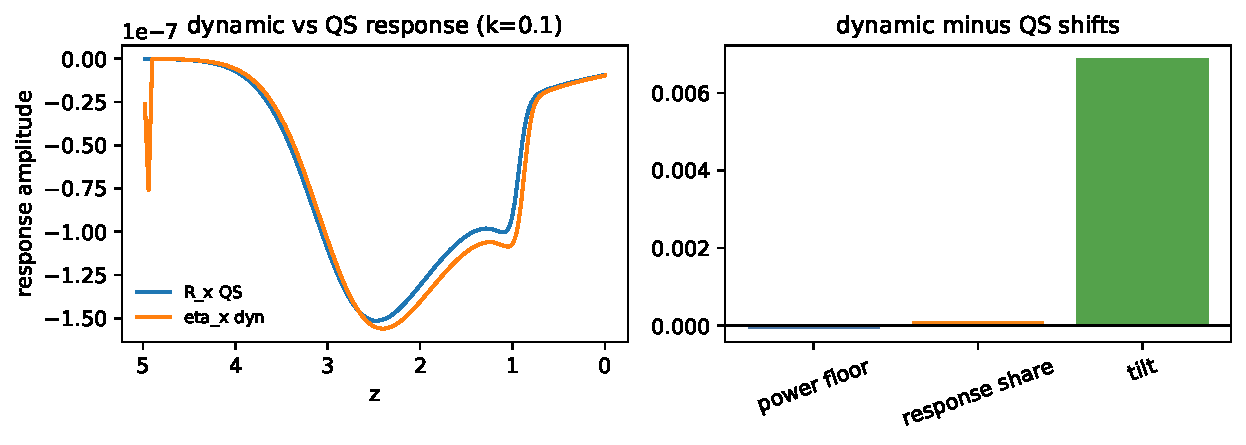
\includegraphics[width=0.95\linewidth]{figures/fig4_dynamic_response.pdf}
\caption{Dynamic-response calibration. The left panel compares the quasistatic
response proxy and the calibrated dynamic response for a representative mode.
The right panel summarizes the small shifts induced by replacing the
quasistatic response with the dynamic replay in the robust source benchmark.}
\label{fig:dynamic_response}
\end{figure}

\subsection{Coupled growth-response solver and Picard feedback}

To test whether the response-derived bridge survives growth integration, we introduced a standalone coupled growth-response solver with absolute variables $(D,V,\delta u,\delta x)$ and a frozen-response three-pass baseline:
\begin{equation}
D_{\rm off}\rightarrow \widehat X^{(0)}\rightarrow D_{\rm on}^{(1)}.
\end{equation}
At direct source insertion $\mu_{\rm eff}=S_{\rm dyn}$, the coupled system is
numerically stable but under-suppresses integrated growth relative to the
dynamic source-level replay, indicating a nontrivial source-to-growth
projection.

We therefore calibrated
\begin{equation}
\mu_{\rm eff}=1+g_{\rm grow}(S_{\rm dyn}-1).
\end{equation}
For the robust benchmark $(p,C_{\rm drain},C_x)=(3.25,0.014,0.015)$ with $(\Gamma_{\rm mult},\alpha_{\rm damp})=(5,30)$, the calibrated point
\begin{equation}
g_{\rm grow}=4
\end{equation}
gives
\begin{equation}
\min_{z,k}P/P_{\mathrm{off}}\simeq0.9511,\quad
\mathrm{tilt}\simeq0.326\%,\quad
\mu_{\rm eff,min}\simeq0.851,\quad
\text{clip}=0,
\end{equation}
which places the coupled replay back into the dynamic-response suppression
window.
The corresponding calibrated-gain benchmark is summarized in
Table~\ref{tab:coupled_gain_calibration}.
\begin{table}[t]
\centering
\begin{tabular}{lcccccc}
\hline
$g_{\rm grow}$ & $f_{\rm resp}(z=0)$ & $\min_{z,k}P/P_{\rm off}$ & $\max_{z}|\mathrm{tilt}|(\%)$ & $\mu_{\rm eff,min}$ & clip & window \\
\hline
1 & 0.1245 & 0.9876 & 0.081 & 0.963 & 0.000 & no \\
4 & 0.1245 & 0.9511 & 0.326 & 0.851 & 0.000 & yes \\
5 & 0.1245 & 0.9392 & 0.408 & 0.814 & 0.000 & no \\
\hline
\end{tabular}
\caption{Calibrated gain benchmark for the robust coupled growth-response replay.}
\label{tab:coupled_gain_calibration}
\end{table}


Finally, a one-step and mini-iteration Picard feedback pilot,
\begin{equation}
D_{\rm off}\rightarrow \widehat X^{(0)}\rightarrow D_{\rm on}^{(1)}
\rightarrow \widehat X^{(1)}\rightarrow D_{\rm on}^{(2)}\rightarrow \cdots ,
\end{equation}
remains stable. In particular, the first update gives
\begin{equation}
\Delta P_{\min}\simeq1.45\times10^{-4},\quad
\Delta \mathrm{tilt}\simeq7.2\times10^{-4}\%,\quad
\Delta f_{\rm resp}\simeq-1.12\times10^{-3},
\end{equation}
with zero clipping, and subsequent updates remain at comparable or smaller deltas. This supports a feedback-stable calibrated coupled benchmark at the standalone level.
The coupled response-share diagnostic is defined after source-to-growth
projection and should not be numerically identified with the source-level
response share.
The Picard convergence table is summarized in
Table~\ref{tab:picard_convergence}.
\begin{table}[t]
\centering
\setlength{\tabcolsep}{6pt}
\begin{tabular}{lcccc}
\toprule
iteration & $\min_{z,k}P/P_{\mathrm{off}}$ & $\max_z|\mathrm{tilt}|$ (\%) & $f_{\mathrm{resp}}(z=0)$ & clip \\
\midrule
iter1 & 0.9511 & 0.3260 & 0.12448 & 0.000 \\
iter2 & 0.9513 & 0.3253 & 0.12336 & 0.000 \\
iter3 & 0.9513 & 0.3253 & 0.12336 & 0.000 \\
iter4 & 0.9513 & 0.3253 & 0.12336 & 0.000 \\
\bottomrule
\end{tabular}
\caption{Picard convergence pilot for the calibrated robust coupled benchmark ($g_{\rm grow}=4$). Iteration-to-iteration shifts remain at the $10^{-4}$ level in the power-floor metric, with zero clipping.}
\label{tab:picard_convergence}
\end{table}


\subsection{Newtonian-gauge CLASS benchmark and metric diagnostics}

After the standalone coupled replay, we add a Newtonian-first CLASS
implementation layer for the response fields. The patch registers two perturbation
variables $(\delta u,\delta x)$, evolves a relaxation-style response RHS in
Newtonian gauge, and routes the resulting dynamic source factor through the
same final matter-source insertion point used in the source-chain tests. This
implementation is designed as a Newtonian-gauge CLASS implementation and does not claim
synchronous-gauge consistency or full Boltzmann closure.

The first acceptance test is a source-response control. A temporary
half-amplitude source multiplier with
$\mu_{\rm eff}=0.5$ gives
\[
P_{\rm ctrl}/P_{\rm ref}=0.25,
\]
as expected for a source-level amplitude multiplier squared. A drain-only run
with
\[
S_{\rm dyn}=1-C_{\rm drain}A_x,\qquad
\mu_{\rm eff}=1+g_{\rm grow}(S_{\rm dyn}-1)
\]
gives $P_{\rm drain-only}/P_{\rm ref}\simeq0.8911$, confirming that the background
activation $A_x$ reaches the final $mPk$ source insertion point. Runs with the closure
disabled or with $C_{\rm drain}=C_x=0$ preserve baseline parity.

The dynamic response channel is then normalized online. At the bounded
Newtonian-gauge benchmark,
\[
\Gamma_{\rm mult}=0.005,\qquad X_{\mathrm{norm,mult}}=7\times10^7,
\]
the dynamic replay gives
\[
P_{\mathrm{geo}}\simeq0.9039,\qquad
P_{\min}\simeq0.8896,\qquad
P_{\max}\simeq0.9351,\qquad
\mathrm{tilt}\simeq3.46\%.
\]
A local refinement at
\[
X_{\mathrm{norm,mult}}=1.5\times10^8
\]
reduces the residual scale dependence to
\[
P_{\mathrm{geo}}\simeq0.8971,\qquad
P_{\min}\simeq0.8896,\qquad
P_{\max}\simeq0.9116,\qquad
\mathrm{tilt}\simeq1.61\%,
\]
with $\mu_{\rm eff}\simeq0.9440$--$0.9454$. A local envelope over
$\Gamma_{\rm mult}\in\{0.003,0.005,0.007\}$ and
$X_{\mathrm{norm,mult}}\in\{1.0,1.2,1.5,1.8,2.0\}\times10^8$ gives $15/15$
local-envelope successes and $6/15$ target-$2\%$ successes. This defines the
Newtonian-gauge CLASS response benchmark.

The metric channel is treated separately as a diagnostic numerical-coupling
audit. We map the available Newtonian-gauge metric access points, wire
metric-lambda hooks into the response helper, and verify that all zero-lambda
metric configurations preserve the fiducial Newtonian-gauge benchmark. The
metric-source scaling and placement ladder is retained as a diagnostic check:
the \texttt{Hconf\_inv2} rescaling restores matched-grid pointwise
reversibility in the audited trace ladder, while inside-bracket placement is
kept as the minimal-change default. This remains an implementation check and
does not validate physical nonzero metric forcing.

The metric-on tests sharpen the boundary. With metric terms enabled, the
metric-on-zero branch preserves the fiducial benchmark, and finite
tiny/micro-lambda runs satisfy Tier-1 finite-output tests up to $|\lambda|=10^{-5}$.
However, no strict symmetric total bounded nonzero-metric window is found.
An incremental audit relative to the metric-on-zero branch identifies a
diagnostic micro-window at $|\lambda|=10^{-10}$, motivating
\[
\Lambda_{\rm met}=\frac{|\lambda|}{10^{-10}}.
\]
A normalized CLASS diagnostic test at $\Lambda_{\rm met}\in\{0,0.3,1,3\}$
satisfies the parity and finite-output gates, while the incremental gates pass only at
$\Lambda_{\rm met}=1$. Thus $\Lambda_{\rm met}$ is useful as a normalized
diagnostic coordinate, but not as a monotonic safety parameter or a physical
coupling calibration.

\begin{figure}[t]
\centering
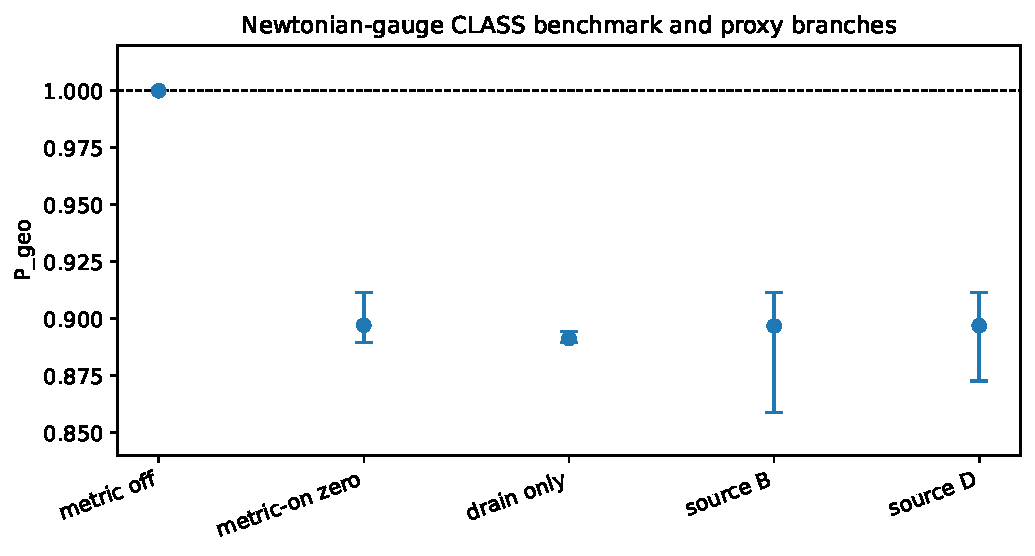
\includegraphics[width=0.78\linewidth]{figures/fig5_newtonian_readiness.pdf}
\caption{Newtonian-gauge CLASS branch and executable source-family proxies.
Points show the geometric mean matter-power ratio relative to the metric-off
reference; bars show the corresponding $P_{\min}$--$P_{\max}$ range. The
source-family branches are executable proxies and do not validate a physical
nonzero metric-forcing model.}
\label{fig:newtonian_readiness}
\end{figure}

\subsection{S8-facing proxy interpretation}
\label{sec:s8_proxy}

To connect the CLASS benchmarks to the low-redshift clustering
target, we translate the geometric mean matter-power suppression into a simple
amplitude proxy,
\[
\frac{S_{8,\mathrm{model}}}{S_{8,\mathrm{ref}}}
\simeq
\sqrt{P_{\mathrm{geo}}}.
\]
This relation is used only as a scale translation. It is exact only for a
scale-independent matter-power suppression. For a scale-dependent suppression,
one would compute the windowed amplitude ratio
\[
\frac{\sigma_{8,\mathrm{model}}}{\sigma_{8,\mathrm{ref}}}
=
\left[
\frac{
\int_0^\infty dk\,k^2 P_{\mathrm{model}}(k,z=0)W_8^2(k)
}{
\int_0^\infty dk\,k^2 P_{\mathrm{ref}}(k,z=0)W_8^2(k)
}
\right]^{1/2},
\]
up to the common normalization factor. The corresponding $S_8$ ratio would
also include $\sqrt{\Omega_{m,\mathrm{model}}/\Omega_{m,\mathrm{ref}}}$ if
the matter-density normalization were varied. In this paper we quote only the
amplitude proxy $\sqrt{P_{\mathrm{geo}}}$. For the final branch, whose residual matter-power tilt is
$\simeq1.61\%$, the geometric-mean proxy is used only as a controlled
amplitude-scale indicator and does not replace a likelihood analysis.

As a direct check on this geometric-mean proxy, we also evaluate the
top-hat-windowed linear amplitude ratio from the archived dense $z=0$
matter-power arrays. The result is shown in
Table~\ref{tab:sigma8_window_check}. This check tests whether
$\sqrt{P_{\rm geo}}$ is a faithful amplitude proxy for the final matter-power
spectra. It is still not a weak-lensing, RSD, CMB, or combined likelihood
analysis.

\FloatBarrier
\begin{table}[t]
\centering
\begin{tabular}{lcccc}
\toprule
Branch & $\sqrt{P_{\rm geo}}$ & $\sigma_8/\sigma_{8,\rm ref}$ & Difference & Note \\
\midrule
reference & $1.000000$ & $1.000000$ & $+0.000e+00$ & reference \\
Newtonian-gauge benchmark & $0.947239$ & $0.949239$ & $+2.000e-03$ & windowed check \\
drain-only & $0.944047$ & $0.944048$ & $+8.246e-07$ & windowed check \\
B proxy & $0.947239$ & $0.949236$ & $+1.996e-03$ & windowed check \\
D proxy & $0.947239$ & $0.949235$ & $+1.996e-03$ & windowed check \\
\bottomrule
\end{tabular}
\caption{Windowed $\sigma_8$ amplitude check from dense $z=0$ matter-power arrays. The $\sqrt{P_{\rm geo}}$ column uses the same $k=0.01$--$0.30\,h\,{\rm Mpc}^{-1}$ band used in the benchmark summaries, while $\sigma_8/\sigma_{8,\rm ref}$ is computed with the top-hat window. This is an amplitude check only, not a likelihood analysis.}
\label{tab:sigma8_window_check}
\end{table}
\FloatBarrier

For the fiducial Newtonian-gauge branch,
\[
P_{\mathrm{geo}}\simeq0.897145,
\qquad
\sqrt{P_{\mathrm{geo}}}\simeq0.947177,
\]
corresponding to an $S_8$-facing proxy suppression of approximately
\[
1-\sqrt{P_{\mathrm{geo}}}\simeq5.28\%.
\]
With the Planck 2018 reference amplitude $S_{8,\mathrm{ref}}=0.831$, this gives
\[
S_{8,\mathrm{proxy}}\simeq0.787,
\]
which is quoted only as a scale indicator, not as a data fit.

We also test two executable source-family proxy branches, denoted B and D,
which represent alternative metric-source operator templates used only for
numerical diagnostics. These branches remain in the same suppression regime.
The source-B control proxy gives
\[
P_{\mathrm{geo}}\simeq0.896795,
\qquad
\sqrt{P_{\mathrm{geo}}}\simeq0.946993,
\]
while the source-D candidate proxy gives
\[
P_{\mathrm{geo}}\simeq0.896930,
\qquad
\sqrt{P_{\mathrm{geo}}}\simeq0.947064.
\]
Both correspond to an approximately $5.3\%$ proxy amplitude suppression and
satisfy the predefined $S_8$-window gates. They do not validate a specific
physical nonzero metric-source operator or physical nonzero metric forcing.

Thus the Newtonian-gauge benchmark produces a controlled matter-power
suppression in the amplitude range relevant to low-redshift $S_8$ comparisons.
A statistical resolution of the $S_8$ tension would require a full likelihood
analysis with weak-lensing, galaxy-clustering, CMB, BAO, and RSD data, including
their nuisance parameters and covariance structure.

As a redshift-aware proxy check, the source-layer suppression is tracked across
the tested redshift range and relaxes smoothly toward unity by $z\simeq2$.
The Newtonian-gauge CLASS branches currently enter the $S_8$ proxy table as
$z=0$ amplitude anchors. This is a ledger-level redshift-shape cross-check, not
a redshift-dependent Newtonian-gauge CLASS validation or a full $f\sigma_8$
prediction.

\begin{figure}[t]
\centering
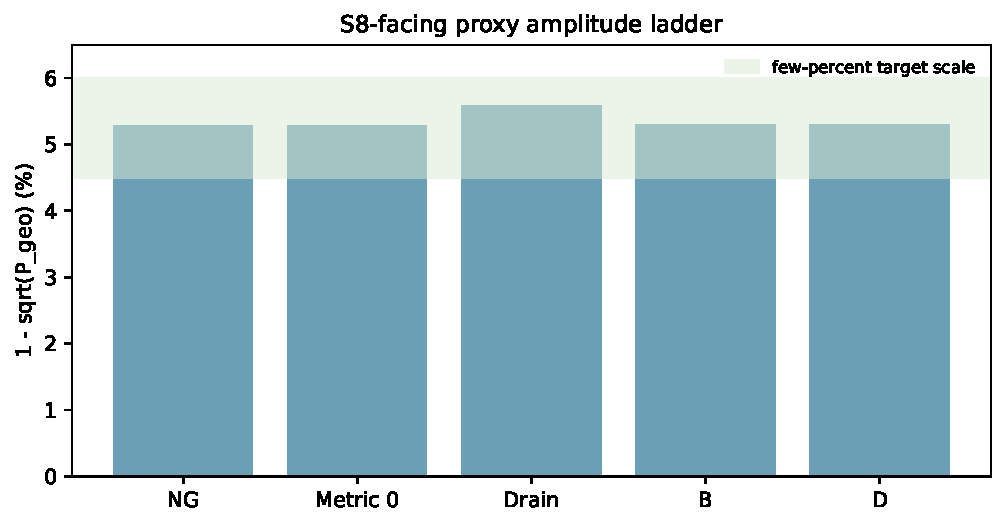
\includegraphics[width=0.78\linewidth]{figures/fig6_s8_proxy_ladder.pdf}
\caption{$S_8$-facing proxy amplitude ladder. The plotted quantity is
$1-\sqrt{P_{\mathrm{geo}}}$ and is used only as a scale translation, not as a
likelihood comparison. The Newtonian-gauge and executable source-family
branches remain near a five-percent amplitude suppression scale.}
\label{fig:s8_ladder}
\end{figure}

\subsection{Compressed observational amplitude comparison}
\label{sec:compressed_s8_comparison}

As a minimal observable-facing check, we compare the amplitude scale of the
CLASS benchmark with published compressed $S_8$ constraints. This is
not a replacement for a DES, KiDS, HSC, RSD, Planck, or combined likelihood
analysis. It only asks whether the matter-power suppression produced by the
selection-fold drain lies in the amplitude range relevant to current
low-redshift clustering measurements.

We use the Planck 2018 base-$\Lambda$CDM value as a reference amplitude,
\[
S_{8,\mathrm{ref}}=0.831,
\]
and define
\[
S_{8}^{\rm comp}
=
S_{8,\mathrm{ref}}\sqrt{P_{\mathrm{geo}}}.
\]
For the fiducial Newtonian-gauge benchmark,
\[
P_{\mathrm{geo}}=0.897145,
\qquad
\sqrt{P_{\mathrm{geo}}}=0.947177,
\]
which gives
\[
S_{8}^{\rm comp}\simeq0.787.
\]
This value lies in the same amplitude range as the low-redshift weak-lensing
constraints from DES Y3, KiDS-1000, and HSC-Y3, while remaining below the
Planck reference amplitude by construction.
The windowed check in Table~\ref{tab:sigma8_window_check} shows that this
geometric proxy agrees with the top-hat-windowed amplitude ratio at the
quoted benchmark level. The corresponding windowed value differs only at the
few-$10^{-3}$ level and does not change the compressed comparison.

The Planck point is used only to set the reference amplitude and is not
included as an independent low-redshift likelihood point. We do not assign a
compressed $\chi^2$ to the comparison, because doing so would obscure the
absence of tomographic kernels, nonlinear modeling, covariance matrices, and
nuisance marginalization.

The compressed comparison shows that the benchmark suppression lies in the
amplitude range relevant for low-redshift clustering comparisons. It does not
establish a statistical resolution of the $S_8$ tension, because such a claim
would require redshift-dependent Newtonian-gauge benchmark power spectra,
weak-lensing kernels, nonlinear modeling, nuisance marginalization, covariance
matrices, and a full likelihood pipeline.

\FloatBarrier

\begin{figure}[t]
\centering
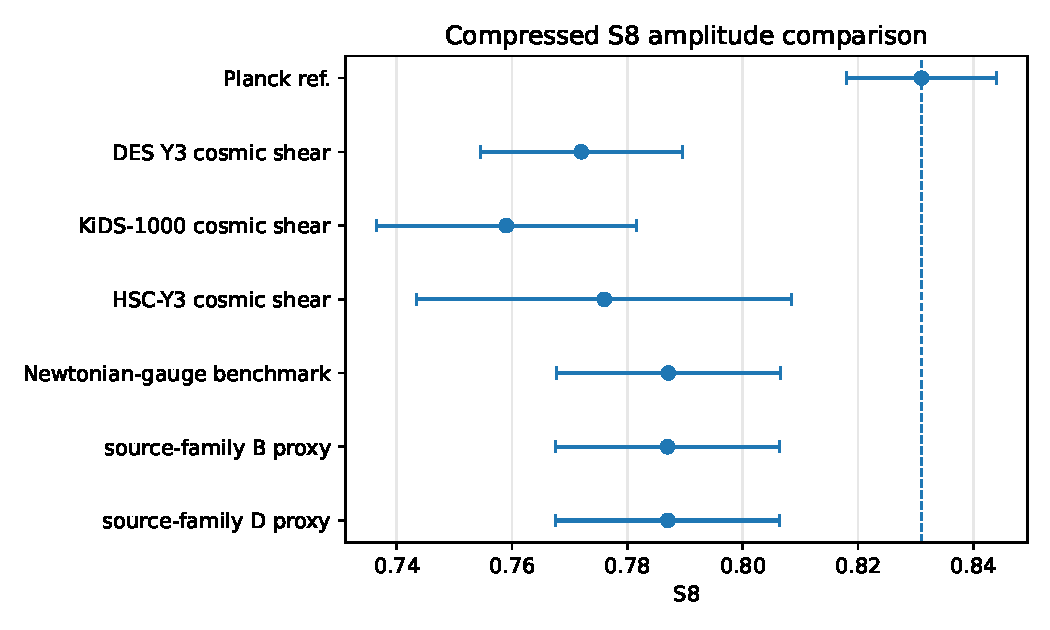
\includegraphics[width=0.92\linewidth]{figures/compressed_s8_comparison.pdf}
\caption{Compressed $S_8$ amplitude comparison. The Planck point is used as
the reference amplitude, while the DES Y3, KiDS-1000, and HSC-Y3 points are
published low-redshift weak-lensing constraints. The benchmark branches are
computed from $S_{8}^{\rm comp}=S_{8,\mathrm{ref}}\sqrt{P_{\mathrm{geo}}}$. The displayed
comparison is an amplitude-scale check only and is not a tomographic
weak-lensing, RSD, CMB, or combined likelihood analysis.}
\label{fig:compressed_s8}
\end{figure}

\begin{table}[b]
\centering
\begin{tabular}{lccc}
\toprule
Compressed constraint & $S_8^{\rm obs}$ & $S_8^{\rm comp}$ & $\Delta S_8$ \\
\midrule
DES Y3 cosmic shear, $\Lambda$CDM-optimized~\cite{DESY3Shear} & $0.772\pm0.018$ & $0.787$ & $+0.015$ \\
KiDS-1000 cosmic shear~\cite{KiDS1000} & $0.759\pm0.022$ & $0.787$ & $+0.028$ \\
HSC-Y3 cosmic shear~\cite{HSCY3Shear} & $0.776\pm0.033$ & $0.787$ & $+0.011$ \\
\bottomrule
\end{tabular}
\caption{Compressed $S_8$ amplitude comparison for the fiducial Newtonian-gauge CLASS branch. The model value is computed as $S_{8}^{\rm comp}=S_{8,\rm ref}\sqrt{P_{\rm geo}}$ using $S_{8,\rm ref}=0.831$. This is an amplitude-scale comparison only, not a weak-lensing, RSD, CMB, or combined likelihood analysis.}
\label{tab:compressed_s8_comparison}
\end{table}

\section{Limitations and interpretation}
\label{sec:limitations}

The present construction is an implementation benchmark, not a cosmological
likelihood model. The source-level insertion tests show that the late-time
selection-drain effect can be transmitted to the CLASS matter-power output
with small residual scale dependence. They do not yet constitute a complete
scalar-perturbation implementation.

The Newtonian-gauge branch registers $(\delta u,\delta x)$, verifies the
matter-source insertion point through half-amplitude and drain-only controls,
and produces a bounded final matter-power response. The metric-dependent terms
are treated only as numerical coupling tests. In particular, the
$\Lambda_{\rm met}$ scans establish finite behavior around the metric-on-zero
branch, but do not validate a physical nonzero metric-forcing model or the full
nonzero metric-source operator.

A further limitation is gauge completion. The dynamic response bridge is a
calibrated first-order perturbation-response prototype; the coupled solver is a
standalone growth-response replay; and the final in-code branch is a
Newtonian-gauge benchmark. A gauge-complete Boltzmann treatment would
require Newtonian-to-synchronous consistency, stress-energy closure, and a
covariant perturbation implementation of the coupled $u,x$ sector, comparable
in spirit to complete modified-gravity or screened-scalar implementations
\cite{Khoury2004,Linder2005,HuSawicki2007,Noller2021}.

The $S_8$ interpretation is likewise proxy-level. We translate the
geometric mean matter-power suppression into an amplitude proxy through
$S_{8,\mathrm{model}}/S_{8,\mathrm{ref}}\simeq\sqrt{P_{\mathrm{geo}}}$ and record
a redshift-aware ledger using the earlier source-layer redshift stability. We
include only a compressed $S_8$ amplitude comparison against published
low-redshift constraints. This comparison is useful for checking the scale of
the effect, but it does not use the DES, KiDS, HSC, RSD, or Planck
\cite{Planck2018} likelihoods, and it does not include tomographic kernels,
nonlinear corrections, baryonic feedback, intrinsic alignments, covariance
matrices, or nuisance-parameter marginalization. It also does not constitute a
full $f\sigma_8$ prediction or a fit to SH0ES \cite{SH0ES}.
The dense $z=0$ spectra archived with this release support the direct
top-hat-windowed amplitude check in Table~\ref{tab:sigma8_window_check}. A
redshift-dependent Newtonian-gauge power-spectrum validation remains future
work.

Finally, any likelihood-level test would require redshift-dependent
Newtonian-gauge benchmark
power spectra, weak-lensing or RSD data vectors, covariance matrices,
nuisance-parameter marginalization, nonlinear scale treatment, and a consistent
prior set. Such an analysis would also require an implementation suitable for
standard sampling pipelines such as MontePython and Cobaya
\cite{MontePython,Cobaya}. These requirements define the likelihood pipeline
needed for a future analysis. The present claim is therefore limited to a controlled
Newtonian-gauge CLASS benchmark with an $S_8$-facing proxy amplitude at the
amplitude range relevant to low-redshift comparisons.

\section{Conclusion}

We have developed a two-field selection-fold dark-drain mechanism for
late-time matter-power suppression. The mechanism is driven by a fold
transition in a selection branch variable $u$, which entrains a physical scalar
$x=\theta/M_{\rm Pl}$ and modulates the cold-dark-matter mass through
$m_c(x)=m_{c0}\exp[-\beta_x(x-x_{\rm ini})]$. This produces a late-time drain
of the cold-dark-matter density and motivates an $S_8$-facing suppression of
linear matter power.

The calculation proceeds from the background bridge to the source-layer
insertion, response replacement, coupled growth replay, and Newtonian-gauge
CLASS branch. The CLASS background bridge matches the reconstructed Friedmann
branch with sub-percent expansion residuals and a derivative-level consistency
check at the $7.68\times10^{-10}$ level. The source-layer insertion verifies
that the final CLASS $mPk$ source insertion point is controllable, including a
source-multiplier control with $P_{\mathrm{on}}/P_{\mathrm{off}}=0.9604$ and
negligible tilt. The response-derived quasistatic kernel, calibrated dynamic
replacement, and standalone coupled growth-response replay preserve the stable
suppression window and remain stable under local sensitivity and
Picard-feedback tests.

The Newtonian-gauge CLASS implementation registers Newtonian response variables
$(\delta u,\delta x)$ and transmits the dynamic source to final matter power.
The fiducial Newtonian-gauge branch gives
$P_{\mathrm{geo}}\simeq0.8971$,
$P_{\min}\simeq0.8896$, $P_{\max}\simeq0.9116$,
$\mathrm{tilt}\simeq1.61\%$, and
$\mu_{\rm eff}\simeq0.9440$--$0.9454$. Metric-lambda hooks preserve the
zero-lambda benchmark and support finite diagnostic numerical coupling, but no physical
nonzero metric-forcing validation is claimed.

The resulting matter-power suppression corresponds to a roughly five-percent
$S_8$-facing amplitude shift under the proxy mapping
$S_{8,\mathrm{model}}/S_{8,\mathrm{ref}}\simeq\sqrt{P_{\mathrm{geo}}}$. This places the
effect in the amplitude range relevant to low-redshift $S_8$ comparisons. The redshift-aware
ledger further shows that the earlier source-layer suppression relaxes smoothly
toward unity by $z\simeq2$, while the Newtonian-gauge branches currently
enter the $S_8$ proxy as $z=0$ amplitude anchors.

The redshift relaxation behavior $P/P_{\mathrm{off}}\to1$ at $z\simeq2$ has
been verified for the source-layer bridge. The Newtonian-gauge CLASS benchmark
currently provides the final in-code matter-power spectrum at $z=0$; full
redshift-dependent validation of that branch is left for future work.

A future extension could replace the phenomenological recordability terms in
$U_{\rm sel}$ by microscopic influence-functional kernels
\cite{FeynmanVernon1963,CaldeiraLeggett1983}.

The work deliberately stops at a controlled Newtonian-gauge CLASS benchmark. It does not provide a
gauge-complete Boltzmann closure, a physical validation of nonzero metric
forcing, a specific physical nonzero metric-source operator, a full
$f\sigma_8$ prediction, or a likelihood-level data fit. Its main contribution
is a reproducible bridge from a selection-fold dark-sector mechanism to a
controlled CLASS matter-power suppression benchmark, with explicit scope
boundaries and a likelihood pipeline roadmap.
\begin{acknowledgments}
The author acknowledges the use of CLASS and related open-source cosmology
software infrastructure.
\end{acknowledgments}

\appendix

\section{Reproducibility manifest}

The curated public release accompanying this manuscript contains the \LaTeX{}
source, local table inputs, generated figures, dense $z=0$ matter-power arrays
used for the windowed $\sigma_8$ check, compressed $S_8$ comparison data, and
scripts used to regenerate the plotted summaries. The release is organized as
follows:
\begin{itemize}
\item \texttt{paper/}: manuscript source, bibliography, local tables, and figures.
\item \texttt{data/background/}: background bridge summaries and diagnostic columns.
\item \texttt{data/matter\_power/}: matter-power ratios used in the benchmark figures.
\item \texttt{data/matter\_power\_dense/}: dense $z=0$ matter-power arrays for the reference and benchmark branches.
\item \texttt{data/sigma8/}: windowed $\sigma_8$ amplitude-check table.
\item \texttt{data/s8\_compressed/}: compressed $S_8$ comparison table.
\item \texttt{scripts/}: figure-generation, compressed-comparison, and windowed-amplitude scripts.
\item \texttt{environment/}: package requirements used for plotting and table generation.
\end{itemize}
The package is intended to reproduce the benchmark tables and figures. It does
not include a DES/KiDS/HSC/Planck likelihood pipeline, full Newtonian-gauge
redshift-dependent matter-power arrays, or a gauge-complete Boltzmann
implementation.

\bibliography{references}
\end{document}










